% ****** Start of file apssamp.tex ******
%
%   This file is part of the APS files in the REVTeX 4.2 distribution.
%   Version 4.2a of REVTeX, December 2014
%
%   Copyright (c) 2014 The American Physical Society.
%
%   See the REVTeX 4 README file for restrictions and more information.
%
% TeX'ing this file requires that you have AMS-LaTeX 2.0 installed
% as well as the rest of the prerequisites for REVTeX 4.2
%
% See the REVTeX 4 README file
% It also requires running BibTeX. The commands are as follows:
%
%  1)  latex apssamp.tex
%  2)  bibtex apssamp
%  3)  latex apssamp.tex
%  4)  latex apssamp.tex
%
\documentclass[%
 reprint,
%superscriptaddress,
%groupedaddress,
%unsortedaddress,
%runinaddress,
%frontmatterverbose, 
%preprint,
%preprintnumbers,
%nofootinbib,
%nobibnotes,
%bibnotes,
 amsmath,
 amssymb,
 aps,
%pra,
%prb,
%rmp,
%prstab,
%prstper,
%floatfix,
]{revtex4-2}

\usepackage{graphicx}% Include figure files
\usepackage{dcolumn}% Align table columns on decimal point
\usepackage{bm}% bold math
\usepackage{tikz}

\usetikzlibrary{arrows.meta, positioning, shapes.geometric, calc}

 
%\usepackage{hyperref}% add hypertext capabilities
%\usepackage[mathlines]{lineno}% Enable numbering of text and display math
%\linenumbers\relax % Commence numbering lines

%\usepackage[showframe,%Uncomment any one of the following lines to test 
%%scale=0.7, marginratio={1:1, 2:3}, ignoreall,% default settings
%%text={7in,10in},centering,
%%margin=1.5in,
%%total={6.5in,8.75in}, top=1.2in, left=0.9in, includefoot,
%%height=10in,a5paper,hmargin={3cm,0.8in},
%]{geometry}

\def\gal{{\tt galacticus}~}
\def\tides{{\tt T1DES}~}
\def\nsphere{{\tt NSphere}~}
\def\galns{{\tt galacticus}}
\def\pyh{{\tt PyHalo}~}
\def\pyhns{{\tt PyHalo}}
\def\cat{Caterpillar }
\def\catns{Caterpillar}
\def\symphony{Symphony }
\def\symphonyns{Symphony}
\def\col{{\tt colossus}~}
\def\colns{{\tt colossus}}
\def\astropy{{\tt astropy}~}
\def\astropyns{{\tt astropy}}
\def\subgen{{\tt subgen}~}
\def\subgenns{{\tt subgen}}
\def\sigsub{{$\Sigma_{\mathrm{sub}}$}}
\def\fssigsub{{$f_{\mathrm{s}} \cdot \Sigma_{\mathrm{sub}}$}}
\def\hanetal{\citet{10.1093/mnras/stv2900}~}
\def\hanetalns{\citet{10.1093/mnras/stv2900}}

\newcommand{\note}[1]{\textcolor{red}{\uppercase{#1}}}

\newcommand{\reffig}[1]{Figure \ref{#1}}

\newcommand{\refsec}[1]{Section \ref{#1}}
\newcommand{\refappendix}[1]{Appendix \ref{#1}}
\newcommand{\reftable}[1]{Table \ref{#1}}
\newcommand{\refeq}[1]{Eq. \ref{#1}}

\begin{document}

\preprint{APS/123-QED}

\title{T1DES in SIDM: A New Class of SIDM Subhalo Simulations}%

\author{Charles Gannon}
 \altaffiliation{University of California, Merced, 5200 N Lake Road, Merced, CA, 95341, USA}
 \email{cgannon@ucmerced.edu}
\author{Anna Nierenberg}
 \affiliation{University of California, Merced, 5200 N Lake Road, Merced, CA, 95341, USA}
  \email{annanierenberg@ucmerced.edu}
\author{Andrew Benson}
 \affiliation{Carnegie Observatories, 813 Santa Barbara Street, Pasadena, CA 91101, USA}
\author{Xiaolong Du}
 \affiliation{Department of Physics and Astronomy, University of California, Los Angeles, CA 90095, USA}
\author{Daniel Gilman}
 \affiliation{Department of Astronomy \& Astrophysics, University of Chicago, Chicago, IL 60637 USA}
\author{Ethan Nadler}
  \affiliation{Department of Astronomy \& Astrophysics, University of California, San Diego, La Jolla, CA 92093, USA}
\author{Andrew Robertson}
 \affiliation{The Observatories of the Carnegie Institution for Science, 813 Santa Barbara Street, Pasadena, 91101, CA, USA}
\author{Ryan Keeley}
 \affiliation{University of California, Merced, 5200 N Lake Road, Merced, CA, 95341, USA}


\date{\today}% It is always \today, today,
             %  but any date may be explicitly specified

\begin{abstract}
Dark matter models with self interactions have gained to resolve apparent shortcomings of the LCDM cosmology.
Testing these models of Self Interacting Dark Matter (SIDM) requires accurate modeling the gravothermal evolution of halos under accelerated heat transport facilitated by these interactions.
The picture becomes more complicated for subhalos (halos evolving within the tidal field of the host), as they have their gravothermal evolution altered by tidal physics in addition to any potential dark matter self interaction; many probes of SIDM such as gravitational lensing sample from a halo population that includes subhalos. 
Existing methods of simulating SIDM subhalos are very computationally expensive or make restrictive assumptions on tidal physics.
To address these shortcomings, we present \tides (Tidal 1D Evolution of SIDM subhalos), a new class of 1D SIDM subhalo simulations incorporating realistic tidal physics while maintaining the many orders of magnitude speed up over full 3D SIDM simulations.
We find that under no evaporation the core collapse is accelerated, with nearly $4$ times as many subhalos collapsing compared to isolated counterparts.
%\begin{description}

%\item[use]
%Secondary publications and information retrieval purposes.
%\item[Structure]
%You may use the \texttt{description} environment to structure your abstract;
%use the optional argument of the \verb+\item+ command to give the category of each item. 
%\end{description}
\end{abstract}

%\keywords{Suggested keywords}%Use showkeys class option if keyword
                              %display desired
\maketitle

%\tableofcontents


\section{Introduction}

% Bare bones SIDM introduction
% SIDM Introduction
Cold Dark Matter or CDM has had a long string of successes explaining the largest scales of cosmology, from the cosmic microwave background \citet{planck2020results}  to the spatial and mass function distributions of galaxies \cite{white1978core,white1991galaxy,de2008high,weinberg2015cold}. 
However, recent inferences on the sub-galactic from direct gravitational imaging the potential of lenses such as the jackpot lens (SDSSJ0946+1006) \cite{vegetti2010detection, minor2021unexpected}, B1938+666 and J0946+1006 \cite{tajalli2025sharp} have provided evidence for anomalously dense (high concentration) dark matter halos compared to CDM predictions.
Although these results have been hotly debated and solutions within the CDM framework have been proposed \cite{he2025not}, the intriguing possibility remains that these results hint at physics beyond CDM.
A class of alternate dark matter models with non-negligible self-interaction on the sub-galactic scales, called self-interacting dark matter (SIDM) has been proposed as an explanation of anomalously dense halos inferred in these systems \cite{zhang2025gd}.
In these models, dark matter self-interaction facilitates the conduction of heat within the halo; due to the negative heat capacity of self-gravitating systems, runaway heat transfer can occur leading to the halo gravothermally collapsing, leading to extremely dense collapsed remnants at the end of their evolution (see Refs. \cite{tulin2018dark,adhikari2025astrophysical} for reviews).

% Previous methods & challenges
In this paper we focus on studying core collapse rates of SIDM subhalos; lensing and stellar streams results sample from a population that includes subhalos. 
To infer SIDM constraints, it is important to understand how fast gravothermal collapse may occur given an SIDM model; tidal forces from the host are know to alter core collapse rates \cite{zeng2022core, shah2024abundance, nishikawa2020accelerated, nadler2025sidm, yang2024parametric}. 
Previously there have been 2 main methods to study SIDM subhalos: 3-D N-body simulations (both cosmological \cite{vogelsberger2012subhaloes, rocha2013cosmological, dooley2016enhanced, nadler2020signatures, turner2021onset, ebisu2022constraining, yang2023strong, nadler2025cozmic}  and idealized \cite{kahlhoefer2019diversity, zeng2022core, zeng2023till, zhang2025gd, klemmer2026survival}) and gravothermal fluid modeling \cite{nishikawa2020accelerated, shah2024abundance}; while these have all been fruitful ways of studying SIDM substructure in their own right, they each have significant drawbacks. 
3-D N-body simulations, which are traditionally the primary method of studying dark matter halos are computationally expensive especially in the core collapse regime; tidal mass loss amplifies this challenge by requiring a larger number of particles to resolve the halo initially, often requiring tens of thousands of core hours to properly resolve core collapse  even in idealized simulations. 
Gravothermal fluid models, while much computationally cheaper than 3-D N-body simulations use restrictive assumptions on tidal physics namely approximating tidal stripping as one or more truncations event where mass is abruptly removed from the halo. 
Because of these limitations, accurately predicting the core collapse rates for large samples of halos across different SIDM models remains a challenge. 

% Our method and sections
In this work, we develop \tides (Tidal 1D Evolution of Subhalos): a pipeline to simulate the evolution of idealized SIDM subhalos in 1-D with realistic tidal evolution. 
By simulating subhalos evolution in 1-D, we are able to simulate SIDM physics much more computationally efficiently than the 3D case, resulting in over an order of magnitude speed up in some case enabling previously infeasible exploration of SIDM model space. 
We begin by explaining our methods in \refsec{sec-methods}.
First, we discuss generating a realization of \gal \cite{BENSON2012175} CDM halos in \refsec{sec-realizations} to set the initial conditions for our 1-D simulations and provide a target mass loss histories. 
Next, in \refsec{sec-dynamics} we discuss how we modify the dynamics of the 1-D simulation code \nsphere \citet{kamionkowski2026numerical, kamionkowski2025gravothermal, kamionkowski2026evolution} to include an effective tidal field calculated from a target mass loss history. 
Then in \refsec{sec-sidm} we discuss the SIDM physics implemented in \nsphere along with the several modifications we make for our use case including a dynamic timestep and core collapse termination condition. 
We then discuss the results of our simulations in \refsec{sec-results} and provide a summary and concluding remarks in \refsec{sec-conclusion}.

\section{Methods}\label{sec-methods}

We aim to explore the population level statistics expected of subhalos systems hosted by strong gravitational lenses. 
To accomplish this we develop the \tides pipeline to simulate realizations of SIDM subhalos across various tidal fields and under the influence of a tidal field.
We use a modified version of the 1-D N-body \nsphere code, this provides a large speed up over traditional 3-D N-body simulations; the slowest halos in our pipeline complete in $\sim 600$ core hours while a comparable idealized 3-D SIDM simulation can take $> 10,000$ core hours to complete. 
In this section, we give an overview of the \tides pipeline with a visual diagram given in \reffig{fig:pipeline}.
Our pipeline requires the the mass history, infall properties (i.e scale radius $r_s$, virial radius $r_v$, and time since infall $t_{inf}$) and tidal tracks (i.e $R_{\tt max}(t), V_{\tt max}(t)$) 
\footnote{Tidal tracks are only required for SIDM mode, as they are used in setting the simulation termination conditions}. 
In \refsec{sec-realizations} we discuss generating generating realizations of lens like hosts and their subhalos in \gal to obtain these quantities.
After generating the realizations in \gal we proceed to evolve the halos in CDM mode in our modified version of \nsphere.
While 1-D N-body simulations provide a significant speed up of full 3-D N-body simulations they provide a unique challenge: simulating asymmetric dynamics of a tidal force in 1-D.
Instead of calculating a tidal field directly from the subhalo's orbit, we do a dynamic "first pass" to calculate the force at every timestep required to match a subhalo's mass history; then we rerun the subhalo with a smoothed version of this tidal field. 
We discuss this as well as the dynamics implemented in our simulations in \refsec{sec-dynamics}.
Finally, we run \nsphere in SIDM mode using a smoothed tidal field; we give an overview of the SIDM implementation in \refsec{sec-sidm}.

\begin{figure*}
    \centering
    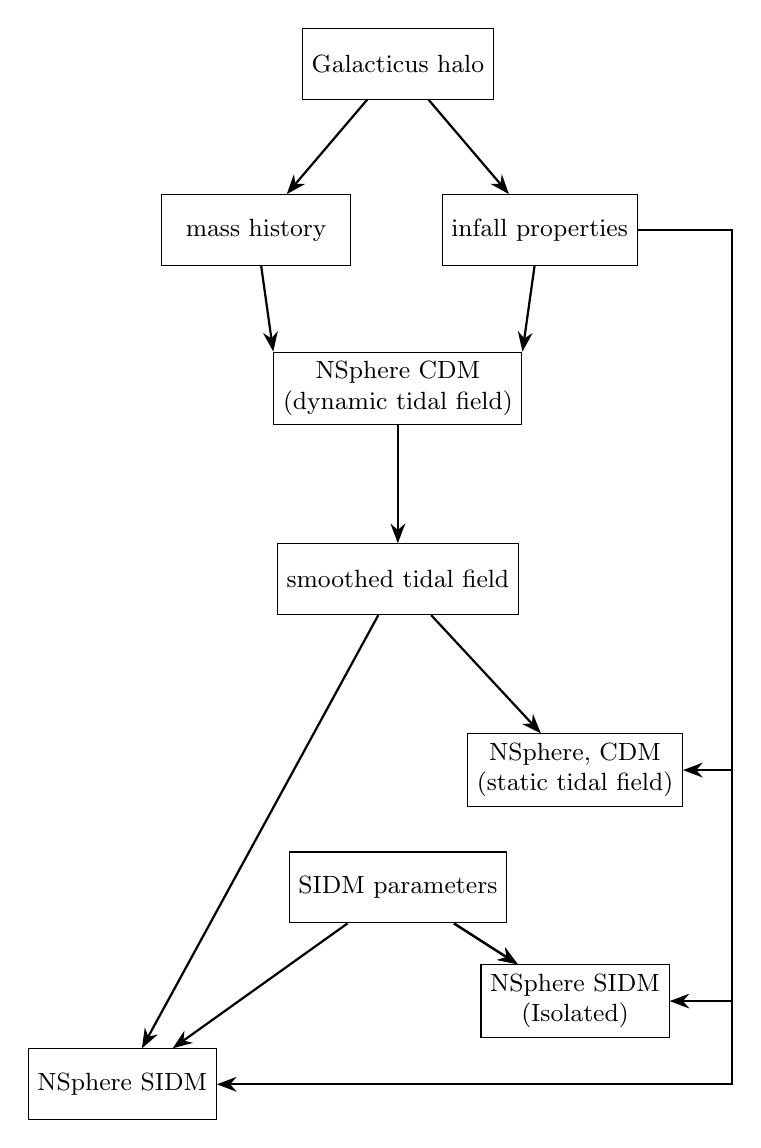
\begin{tikzpicture}[
        node distance=1.2cm and 0.6cm,
        box/.style={
            draw,
            rectangle,
            minimum width=2.0cm,
            minimum height=0.9cm,
            align=center,
            font=\small
        },
        param/.style={
            draw,
            rectangle,
            minimum width=2.4cm,
            minimum height=0.9cm,
            align=center,
            font=\small
        },
        arrow/.style={-{Stealth[length=2.5mm]}, thick},
        every label/.style={font=\footnotesize}
    ]
     
    % Top node
    \node[box] (halos) {Galacticus halo};
     
    % Parameters row (two grouped boxes)
    \node[param, below=1.2cm of halos, xshift=-1.8cm] (mass)   {mass history};
    \node[param, below=1.2cm of halos, xshift= 1.8cm] (infall) {infall properties};
     
    % CDM node
    \node[box, below=3.2cm of halos] (cdm) {NSphere CDM \\ (dynamic tidal field)};
     
    % Tidal field node
    \node[box, below=1.5cm of cdm] (tidal) {smoothed tidal field};
     
    % SIDM node
    \node[box, below=5.5cm of tidal, xshift=-3.5cm] (sidm) {NSphere SIDM};

    % Static tidal field
    \node[box, below=1.5cm of tidal, xshift=2.25cm] (cdm_static) {NSphere, CDM \\ (static tidal field)};

    % SIDM Isolated
    \node[box, below=2.0cm of cdm_static] (isolated) {NSphere SIDM \\ (Isolated)};
    
    % Cross-section node (to the left of tidal)
    \node[box, below=3.0cm of tidal] (sigma) {SIDM parameters};
     
    % Arrows: halo -> parameter boxes
    \draw[arrow] (halos) -- (mass);
    \draw[arrow] (halos) -- (infall);
     
    % Arrows: parameters -> CDM
    \draw[arrow] (mass)   -- (cdm.north west);

    \draw[arrow] (infall) -- (cdm.north east);
     
    % Arrow: infall properties -> SIDM (routed down the right side, entering SIDM from the right)
    \draw[arrow] (infall.east) -| ($(infall.east) + (1.2,0)$) |- (sidm.east);
    \draw[arrow] (infall.east) -| ($(infall.east) + (1.2,0)$) |- (cdm_static.east);
    \draw[arrow] (infall.east) -| ($(infall.east) + (1.2,0)$) |- (isolated.east);
     
    % Arrow: CDM -> tidal field
    \draw[arrow] (cdm) -- (tidal);
     
    % Arrow: tidal field -> SIDM
    \draw[arrow] (tidal) -- (sidm);
    \draw[arrow] (tidal) -- (cdm_static);
     
    % Arrow: sigma/m -> SIDM
    \draw[arrow] (sigma) -- (sidm);
    
    \draw[arrow] (sigma) -- (isolated);
    
    \draw[arrow] (sigma) -- (isolated);
    
\end{tikzpicture}
 
 \caption{
         A diagram of the \tides pipeline simulating a single subhalo.
         The \tides pipeline begins with extracting infall properties ($r_s$, $r_v$, $z_{infall}$) as well as the bound mass of the subhalo as a function of time. 
         Our main results use the \gal galaxy formation model to extract the infall mass properties of the subhalo, however we also include results using properties extracted from N-body simulations. 
         These are used to set the initial conditions of the halo and begin running a first pass of NSphere in "dynamic" tidal field mode. 
         During this run, NSphere calculates a tidal field "in flight" that results in a mass history approximating that of the galacticus halo. 
         After the run, the tidal field is then smoothed on the scale of the dynamical time of the subhalo to remove the rapid variations in the initial calculation of the tidal field.         
         For comparison, we rerun NSphere in CDM mode to get a "replay" of the subhalo's evolution using the smoothed tidal field.
         Then we run NSphere in SIDM mode with the smoothed tidal field.
         Finally, for comparison we run a NSphere SIDM on an isolated halo corresponding to the infall properties of the subhalo.
         }
 \label{fig:pipeline}
\end{figure*}
 

\subsection{Subhalo Realizations}\label{sec-realizations}
We aim to simulate realizations of lensed subhalos in a $10^{13} M_{\odot}$ host in SIDM; our T1DES pipeline requires subhalo properties (mass history, infall properties) as a starting point. To obtain these quantities we simulate subhalo populations we use the semi-analyic galaxy formation model, \gal to generate subhalo populations. Semi-analytic are faster than traditional 3D N-body simulations and allow us to realize subhalo populations quickly. The \gal model is particularly well suited for our use case because of it's recent calibration to high resolution idealized simulations \citep{du2024tidal} and it's extensive and well tested library of dark matter physics. However, we note that our model is not limited to only using subhalo properties obtained using the \gal galaxy formation model. It is possible to use evolutionary histories obtained from other sources such as N-body simulations, which we explore later in this paper.

We give a brief summary of the \gal dark matter models used and then discuss the simulation configurations used and selection criteria for subhalos. First we discuss the discuss the procedure \gal uses to simulate subhalo populations: first, merger trees are generated and then evolved forward in time using a set of analytic and semi-analytic models. Finally, we discuss our simulation parameters and the selection criteria for lensing like subhalos. 

Merger tree generation — We build our \gal merger trees algorithms presented in \citet{cole2000formation} and \citet{parkinson2008generating}. 
The algorithm is works by calculating branching probabilities: step back in time and at each time step calculating branching probabilities using the extended \citet{press1974formation} formalism. 
Using the branching probabilities, a merger tree is then built backwards in time that includes both merger events (infalling halos) and smooth accretion. Halo scale radiis are set using the \citet{ludlow2016mass} and concentrations are set using the \citet{diemer2019accurate} model.

Node evolution — After merger trees are built, our \gal model tracks infalling (subhalos) halos and forward evolves them in time; first subhalo's orbits are initialized, then their orbits and profiles are evolved using a set of analytic models. When a subhalo infalls (a merger event happens) it's orbit is initialized according to the potential of the host. After initialization the subhalo's orbit is evolved forward in time using models for dynamical friction, tidal heating and tidal stripping.  We give a high level overview of these models here: 
\begin{itemize}
    \item Dynamical friction — Dynamical friction causes subhalo orbits to decay; our configuration uses the \cite{chandrasekhar1943dynamical} model with a Columb logaritm $\log \lambda = ?$ tuned to the \citet{grilfen2016caterpillar} simulations. 
    \item Tidal Heating — Interactions with the tidal field of the host dynamically heat the host's dark matter density causing the profile to expand. Our \gal models use the \citet{gnedin1999tidal} tidal heating model tuned to high resolution idealized simulations provided by \citet{du2024tidal}.
    \item Tidal Stripping — Mass outside of the tidal radius is removed by tidal forces. Our \gal models use the \citet{zentner2005physics} tidal stripping model with and is tuned to high resolution idealized simulations provided by \citet{du2024tidal}.
\end{itemize}

Simulation Configuration — Using the \gal model we simulate the subhalo population of 10 lensing like $10^{13} M_{\odot}$ halos.
In this work, we focus on subhalos in the mass range  $10^{9} \leq m / M_\odot \leq 10^{10}$.
Our \gal models have an infall mass resolution of $8.00 \cdot 10^{8}$ and subhalos are destroyed is they lose more than $90\%$ times their infall mass due to tidal effects.
For our T1DES simulations, we select "lensing like" subhalos: subhalos with a $20 < r_{\tt 2d} / {\tt kpc} < 50$ projection of the center of the host.
These are subhalos that are likely to be sampled from in a strong lensing study. We also exclude subhalos that have been in the subhalo for less than $1.0 {\tt Gyr}$ as they likely have not completed a single orbit. 
Subhalos within x kpc of the host are destroyed. 

For this analysis we only first-order substructure; that is subhalos that are field halos until they fall into the primary host. This contrasts with 2nd order and higher subhalos which are accreted into intermediate halos before infalling into the host.
\begin{itemize}    
    \item Extreme mass histories --- \gal often predicts extreme early mass loss histories for 2nd order and higher subhalos. This is likely an artifact of the way \gal handles the orbits of these subhalos; these extreme mass histories characterized by rapid early mass loss when accreted into the first host and much steadier mass loss when accreted into the final host. This is likely an artifact due to how our \gal handles subhalo orbits: with 2nd order substructure disabled some subhalos rapidly loosing mass on first accretion then when the first host is acrreted, the subhalo abruptly stops loosing mass to it's first host and begins loosing mass to the it's new host. Our pipeline often disagrees with \gal on the internal properties of these subhalos. We leave further investigation to future work. 
    \item Simplifying our analysis --- In our \gal models, 2nd order subhalos have 2 distinct orbits: one in the precursor subhalo and one in the primary host; this would significantly complicate our analysis. For the purpose of this work, we study the simpler case of 1st order substructure and leave these complexities to future work. 
\end{itemize}
Due to these complications, we leave exploring extending the \tides pipeline to higher order substructure to future work. 

 \subsection{Gravitational Dynamics}\label{sec-dynamics}
  We modify the 1D N-body code \nsphere to include the influence of a linear tidal force. The tidal dynamics experienced by a subhalo's particle are asymmetric in our subhalo's coordinate frame. 
To model tidal physics in our spherically symmetric simulations, we need to choose an effective tidal field; we choose our tidal field to match the target halo's bound mass loss rate. 
Choosing a tidal field strength can be thought of as choosing a tidal radius.
We would expect mass outside the Roche volume of the subhalo to be lost on order the dynamical time of the subhalo. 
Our choice to match the mass loss history of the subhalo is natural: where the effective tidal force dominates the gravitational subhalo, the subhalo loses mass; this forms a volume () outside of which mass is being lost; we choose a tidal radius enclosing approximately the same mass as this volume. 

  Under the influence of gravity and a linear tidal force with the assumption of spherical symmetry, the acceleration of $i$th shell is 
 \begin{equation}\label{eq_dynamics}
     \ddot{r}_{i} = - \frac{G M(< r_i)}{r_i^2} + \frac{l_i^2}{r_i^3} + f_t r_i
 \end{equation}, 
 where $r_i$ is the distance from to center of the subhalo from the $i$th particle, $l_i$ is the angular momentum per unit mass on each particle, $M (< r_i)$ is the mass enclosed by radius $r_i$ and $f_t$ is the linear tidal field.  
 For each \tides halo, we calculate a aim to calculate a tidal field to approximate the mass loss history of it's corresponding galacticus subhalo.
 Following \cite{du2024tidal}, outside the tidal radius, we assume the rate of mass loss to be on the dynamical timescale of the halo   
\begin{equation}\label{eq_du_2024_massloss}
 \frac{dM_{\text{sub}}}{dt} = - \alpha_s \frac{M_{\text{sub}}(> r_t)}{T_{\text{dyn}}}				
\end{equation} 
where $M_{\text{sub}}$ is the gravitationally bound mass of the subhalo, $\alpha_s$ controls the tidal stripping rate, $r_t$ is the tidal radius, and $T_{\text{dyn}} = 2\pi\sqrt{r_t^3 / 16GM_{\text{sub}}(<r_t)}$ is the dynamical time of the subhalo.
For a \tides subhalo with bound mass $M_{T}$ at time $t$ we solve the following equation 
\begin{equation}\label{eq_du_2024_rt}
        -\alpha_s \frac{M_{\tt T}(t, > r_t)}{T_{\tt dyn}} = \min \left \{ \frac{M_{\tt g}(t + \Delta t) - M_{\tt T}(t)}{\Delta t}, 0 \right\}
\end{equation} 
to calculate a tidal radius that results the reduction in mass to the mass galacticus halo, $M_{g}$ at time $t + \Delta t$
; we do not allow the right hand side of the equation to be greater than zero since the subhalo can only lose mass.
Due to the self-correcting feedback introduced by the right hand side of \refeq{eq_du_2024_massloss}, we find our simulations are fairly insensitive to our choice of $\alpha_s$, we choose $\alpha_s = 4$ to match \cite{du2024tidal}. 
The tidal force and gravitational force balance at the tidal radius, $r_t$; assuming a linear tidal force $F_t \propto r$ the tidal field corresponding to a tidal radius $r_t$ is 
\begin{equation}\label{tidal_field}
 f_t = \frac{G M(< r_t)}{r_t^3} 
\end{equation}.
Since our prescription can produce large jumps in the tidal field, we smooth the tidal field on order the the dynamical time of the subhalo, $T_{dyn}$ in post processing; we find that running with the smoothed tidal field using a gaussian filter with width $1/10 T_{dyn}$ produces nearly identical halo evolution to the original run.

\begin{figure}\label{fig-history-sample}
    \includegraphics[width=\linewidth]{figures/rmax_vmax_mbound_t1h3645.pdf}
    \caption{
              The evolutionary history of an example CDM \tides subhalo and it's \gal counterpart. 
              We show the bound mass history, $M_{\tt bound}$ as well as the internal properties of the subhalo, $R_{\tt max}$ and $V_{\tt max}$ (see \refeq{eq-vmax}).               
              Each sudden drop in the mass history corresponds to a peri-centric passage of the subhalo, this subhalo completes 10 pericentric passages in it's 7Gyr evolution within the host, losing $\sim 90\%$ of it's mass since infall.
              Results from both \tides stages are shown: results from the \tides dynamic stage, where the is dynamically calculated as well as the results from the \tides dynamic stage, where we rerun with the dynamically calculated tidal field smoothed by a gaussian kernel.
              We note that while our model calculates a tidal field to match the provided \gal mass history, it is not tuned to match the internal $R_{\tt max}$ and $V_{\tt max}$ properties; even so it is in good agreement with \gal for nearly all halos.               
     }
\end{figure}

\begin{figure}\label{fig-tidal-tracks}
    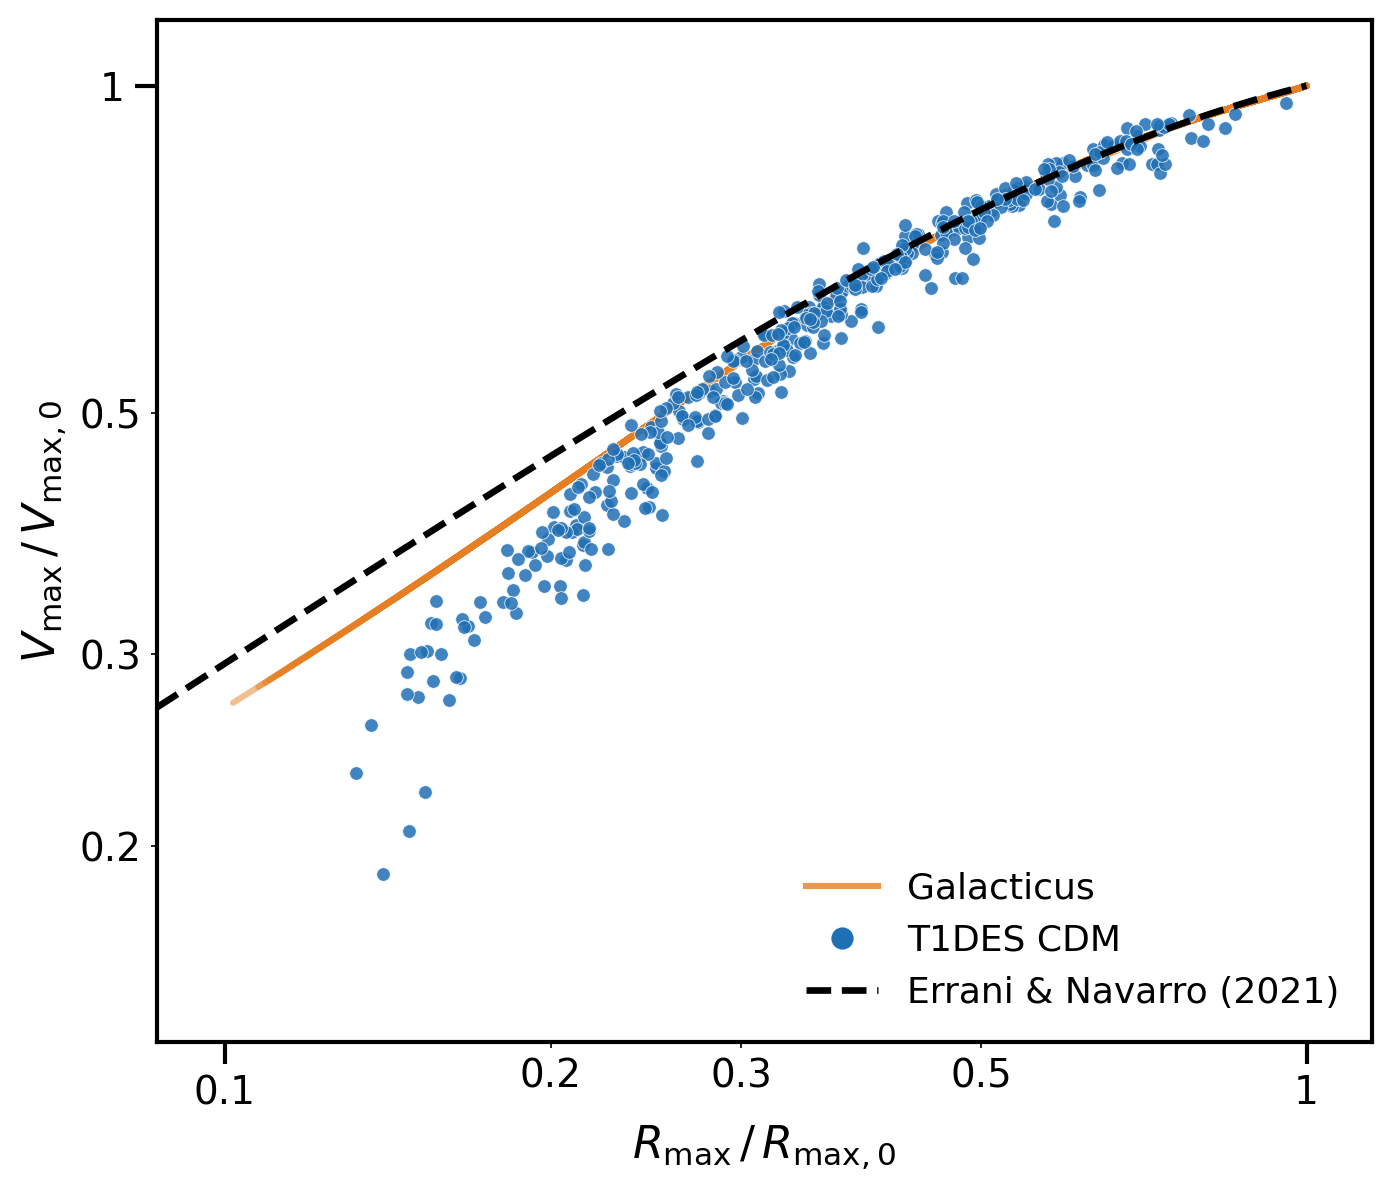
\includegraphics[width=\linewidth]{figures/tidal_tracks_normalized_errani_scratch.png}
    \caption{
              We plot the normalized tidal tracks from our \tides CDM smoothed stage simulations, our \gal models and from the empirical \citet{errani2021asymptotic}. For each subhalo in our suite, we plot the $R_{\tt max} / R_{\tt max,0}$ and $V_{\tt max} / V_{\tt max,0}$ at the subhalo's apocenter where $R_{\tt max,0}$ and $V_{\tt max,0}$ are the initial $R_{\tt max}$ and $V_{\tt max}$ of the subhalo at apocenter. We plot the Normalized tidal tracks from \gal, \tides and predictions . When properly normalized, CDM tidal tracks are expected to follow a near universal relation. We find general good agreement on the tidal track level between our simulations; with slight disagreement for low $R_{\tt max}$ and $V_{\tt max}$. 
     }
\end{figure}



We show the evolutionary history for both stages of our \tides model as well as it's \gal counterpart in \reffig{fig-history-sample}.
%We discuss how the evolutionary history of a wider sample of subhalos in \refappendix{apdx-tidal} and discuss the differences between \gal mass histories and those predicted by high resolution idealized N-body simulations, and discuss the sharp "staircase" mass histories predicted by \gal but not seen in N-body simulations.
Due to our choice of tidal field, in CDM, our model is in excellent agreement with the bound mass history of both \gal and 3D idealized N-body simulations. 
In addition, we also compare our model's prediction for the internal properties $R_{\tt max}$ and $V_{\tt max}$ curves to \gal and predictions from idealized N-body simulations with the caveat that our model sometimes overshoots the mass loss from \gal simulations.
\reffig{fig-tidal-tracks} shows an important diagnostic for our simulations: we plot the normalized tidal tracks, $R_{\tt max} / R_{\tt max,0}$ vs $V_{\tt max} / V_{\tt max,0}$ for each subhalo at apocenter. 
We include \tides CDM model, along with results from out \gal model and the empirical \citet{errani2021asymptotic} model; 
These curves are particularly important as they are the scale on which SIDM evolution happens \cite{yang2024parametric}.
When properly normalized, CDM tidal tracks are expected to follow a near universal relation.
We find general good agreement on the tidal track level between our simulations; with slight disagreement for low $R_{\tt max}$ and $V_{\tt max}$, however we note that this discrepancy is nearly as large as the difference between the \gal model and \citet{errani2021asymptotic}.
Additionally, the \gal tidal tracks results form nearly a perfect curve with very little scatter; while our \tides model has more significant scatter: likely due to the noise discrete noise inherent to N-body simulations.
While our model is not specifically calibrated to match these curves, our model is in reasonable agreement with both the results from \gal and 3D N-body simulations.

\subsection{SIDM Physics}\label{sec-sidm}
Here, we give an overview of the SIDM physics implemented in our simulations; we use the default NSphere SIDM implementation with the addition of an adaptive timestep. We discuss our choice of cross sections and finally, we discuss the termination conditions we impose on the simulation and how we define core collapse.

SIDM Scattering --- 
The probability of the $i$ th particle scattering in the simulation within some time scale $\Delta t$ is evaluated by summing over all particles from $r_1$ to $r_1 + \Delta r_i$
\begin{equation}\label{eq-scatter-probability}
    P_1(r_1, v_1, c_{\theta_1}) = \frac{\Delta t}{2} \left(\frac{m_p}{4\pi r_1^2 \Delta r}\right) \sum_{r_i=r_1}^{r_1+\Delta r} \sigma_{\text{eff}}(v_{\text{rel},i}) v_{\text{rel},i},
\end{equation}
where $m_p$ is the particle mass, $v_{rel}$ is the relative velocity between the two particles and $\sigma_{\text{eff}}(v_{\text{rel}}) = \frac{1}{m}\int_{-1}^{1} d\cos\alpha \, (d\sigma/d\cos\alpha)$ is the total cross section with $m$ being the mass of the elementary particle,.  
We use the default NSphere bin width, $\Delta r = r_{i_i + j} - r_{i_1}$ with $j_{1} = 10$.

After particles scatter, their kinematics must be calculated. When two identical particles with velocities $\mathbf{v_1}$ and $\mathbf{v_2}$ scatter,  the Center of Mass (COM) frame has velocity $\left ( \mathbf{v_1} + \mathbf{v_2} \right ) / 2$. COM frame, the particles have outgoing velocities $v_{\tt cm 1}$ and $v_{\tt cm 2}$ both having equal magnitudes to half the incoming relative velocity $v_{\tt rel, 2} / 2$ and offset by angle $\alpha$. We assume isotropic scattering; therefore, the cosine of the scattering angle, $\cos \alpha$ is chosen uniformly from $-1$ to $1$ and the polar angle $\phi_f$ around $v_{\tt rel, 2}$ is chosen uniformly on the interval $0$ to $2 \pi$. After the velocities have been calculated, they are projected into the halo frame and saved for the next timestep.

Timestep --- 
The key timescale for SIDM evolution is the scattering time, $t_{\tt scatter} = [\rho \sigma_{\tt m} v]^{-1}$.
To accurately model this evolution, the chosen timestep of the simulation, $\Delta t_{step}$ must be much less that the scattering time ($\Delta t_{\tt step}< t_{\tt scatter}$)
Therefore, the size of the timestep sets the maximum density (and velocity) that can be resolved by the simulation; by default, \nsphere implements a constant timestep, $\Delta t_{\tt step} = C$.
In this method, the fixed timestep size is set by choosing a maximum resolvable density. 
However, this is inefficient as a very small timestep must be chosen to resolve the high density of core collapse and the halo will only reach this density at the very end of it's evolution. 
Instead, we implement an adaptive timestep; we choose the size of the adaptive timestep based on the probability of two particles scattering in the previous timestep, $P_{\tt i}$ (see \refeq{eq-scatter-probability})
\begin{equation}
    \Delta t_{\tt step,n+1} = \max \left \{ \epsilon \cdot  \frac{\Delta t_{\tt step, n}}{\max \left \{ P_{\tt i} \right \}} , \Delta t_{\tt step, min} \right \}
\end{equation}
where we ensure that if the particles maintained the same scattering probability in the next timestep, the maximum scattering probability would be $\epsilon$.
For our simulations, we find good convergence with $\epsilon = 1.0 \cdot 10^{-4}$. 
Taking the minimum of all particle scattering probabilities can result in very small time steps, for instance due to a single pair of particles that are highly likely to scatter in the next timestep; we prevent these extremely small timesteps by implementing a timestep floor $\Delta t_{\tt step, min}$. 
We set the timestep floor proportional to the maximum density we expect to resolve in the simulation, $\Delta t_{\tt step, min} = [\bar{\rho}_{\tt max}(< R_{\tt max}) \sigma_{\tt m} \max \left \{ V_{\tt max} \right \}]$ where $\bar{\rho}_{\tt max}(< R_{\tt max})$ is the termination density of our simulations and $V_{\tt max}$ is the circular velocity predicted for the target halo (in this case, we use the result from \gal model).
We conveniently use $\left \{ V_{\tt max} \right \}$ as the characteristic velocity because for the cross-sections studied and the termination condition we use, the termination $V_{\tt max}$ in SIDM remains slightly higher than (maximum $\sim 20 \%$ more) or less than the $\max \left \{ V_{\tt max} \right \}$ in CDM due to tidal stripping. 

Cross Section --- 
For this work, we explore a constant cross section per unit mass $\sigma_{\tt eff}$ and run simulations with 5 cross-sections $\sigma_m / ({\tt cm^2 / g}) = 5, 10, 25 \text{ and }50$ and assume a SIDM model with elastic scattering. 
In this work we focus on core collapsed halos; strong lensing probes are most sensitive to core collapsed halos and insensitive to cored halos \cite{gilman2021strong}.  
Constant SIDM cross sections constraints from clusters \cite{eckert2022constraints,sagunski2021velocity,andrade2022stringent} and dwarf and satellite galaxies \cite{ando2025stringent, correa2021constraining} constrain constant cross section SIDM models to cross sections below $\sigma_m < 1 {\tt cm^2 / g }$ which is lower cross section than considered in this work, and below the cross sections we find subhalos collapsing in our simulations.
In our simulations, we do not consider SIDM particle interactions with the host; if SIDM interactions with host particles are not suppressed by (as is the case with a truly constant cross section SIDM models) subhalos are not expected to collapse due to evaporation \cite{zeng2022core}. 
Therefore, the constant cross sections in this work should be considered as an illustrative case study rather than something that is expected to be probed by strong lensing; mappings exist from velocity dependent cross sections to constant "effective" cross sections, which allow mapping our work onto velocity dependent cross section models, see References \cite{yang2022gravothermal, yang2023gravothermal, outmezguine2023universal}.
Finally, we note many velocity-dependent cross sections considered in lensing analysis such as parametric cross section form considered in \cite{gilman2021strong} asymptotes to a nearly constant cross section in the low velocity regime; these results can be viewed as exploring that regime: near constant cross section at low velocities and highly suppressed cross section on the scale of the host. 

Core Collapse and Termination Conditions --- 
Unlike field halos, the characteristic scale of subhalos may greatly decrease over time due to the effects of tidal stripping; to define core collapse we cannot simply choose a density threshold value at a fixed radius. 
Instead, we use the $R_{\tt max}$ as the characteristic scale, where $R_{\tt max}$ is the radius at which the maximum circular velocity $V_{\tt max}$ 
\begin{equation}\label{eq-vmax}
    V_{\tt max} = {\tt Max}\left \{ \sqrt{\frac{G M(<r)}{r}} \right \} = \sqrt{\frac{G M(<R_{\tt max})}{R_{\tt max}}}
\end{equation}
occurs.
From \refeq{eq-vmax}, it follows that the average density within $R_{max}$, $\bar{\rho}_{\tt max} \left(< R_{\tt max} \right)$ is
\begin{equation}
 \bar{\rho}_{\tt max} \left(< R_{\tt max} \right) = \frac{3}{4 \pi G} \left( \frac{V_{\tt max}}{R_{\tt max}} \right)^2 
\end{equation}. 
We define a subhalo as core collapsed and terminate with when the density within $R_{\tt max}$ is 
\begin{equation}\label{eq-collapse-threshold}
 \bar{\rho}_{\tt max} \left (< R_{\tt max} \right ) >= n\frac{3}{4 \pi G} \left( \frac{\max{\{V_{\tt max}(t)\}}}{\min{ \{ R_{\tt max}(t) \} }} \right)^2  
\end{equation}. 
where $n > 1$ is an arbitrary factor that determines how deep into core collapse we resolve; for this work we chose $n = 10$.

\section{Results}\label{sec-results}

Here we discuss results from our suite of \tides simulations. First, we compare results of subhalos with their isolated counterparts. We find that subhalos core collapse rates are strictly accelerated by the presense of a tidal field when compared to their isolated counterparts. Next, we compare our results to previous work including the \citet{yang2024parametric} parametric model for core collapse.  We find good agreement with the parametric model and a similar order of magnitude core collapse acceleration when compared to \citet{nadler2025sidm}.

Core Collapse Acceleration ---  \reffig{fig-collapse} shows the the cross section per unit mass vs the core collapse fraction, the number of total core collapsed subhalos divided by total number of subhalos, $f_{\tt collapse}$  for our \tides simulations compared to the predictions from \cite{yang2024parametric} parametric model.
We compare our tides subhalos run with a tidal field (\tides SIDM stage) to their counterparts ran without a tidal field using the same initial conditions (\tides isolated stage). 
We find that all isolated halos that collapse also collapse also collapse when run with a tidal field; the influence of a tidal field in our simulations strictly accelerates core collapse rate.  
However, we note that our results assume evaporation is negligible; for SIDM models where this is not the case, core collapse may delayed instead of accelerated.
We find roughly similar acceleration rates to \citet{nadler2025sidm} who compared the predicted core collapse rates for populations of isolated halos to subhalos in a SIDM model with a velocity dependent cross section; at $\sigma_{m} = 25 {\tt cm^2 / g}$ nearly $4$ times as many subhalos collapse when compared to their isolated counterparts and at $\sigma_{m} = 50 {\tt cm^2 / g}$ ($46\%$) nearly $2$ times as many subhalos collapse. 
We find subhalo collapse for a cross section as low as $\sigma_{\tt m} = 10 {\tt cm^2 / g}$; at this cross section around $5\%$ of the subhalos in our models collapse while none of their isolated counterparts do. 
For some SIDM models it may be possible that a non-negligible fraction of subhalos core collapse before any field halos do, due to accelerated core collapse from a tidal field. 


Comparison with previous results --- 
\reffig{fig-collapse} also shows the collapse fraction $f_{\tt collapse}$, for our \tides simulations compared to the predictions from the \citet{yang2024parametric} model; for this model, we show results obtained by integrating over the the tidal tracks from \gal  and from the \tides CDM. 
We find our \tides model is fairly consistent with the predictions from the \citet{yang2024parametric} model, though our \tides model may predict slightly higher fractions of core collapsed halos. 
Interestingly our the \citet{yang2024parametric} predictions integrating over the \gal tidal tracks appear to agree slightly better with our \tides predictions than the the results obtained by integrating over the \gal tidal tracks.
We also note that the core collapse definition between our \tides model and the \citet{yang2024parametric} model is different; \citet{yang2024parametric} defines core collapse as $\tau > 0.75$ while we use the $R_{\tt max}$ based density threshold given by \refeq{eq-collapse-threshold}.
However, the difference in definitions likely only impacts the number of collapsed halos slightly; the final core collapse happens on short timescale compared to the entire SIDM evolution.
We leave a more detailed comparison and investigating these possible discrepancies to future work.

\begin{figure*}
    \centering
    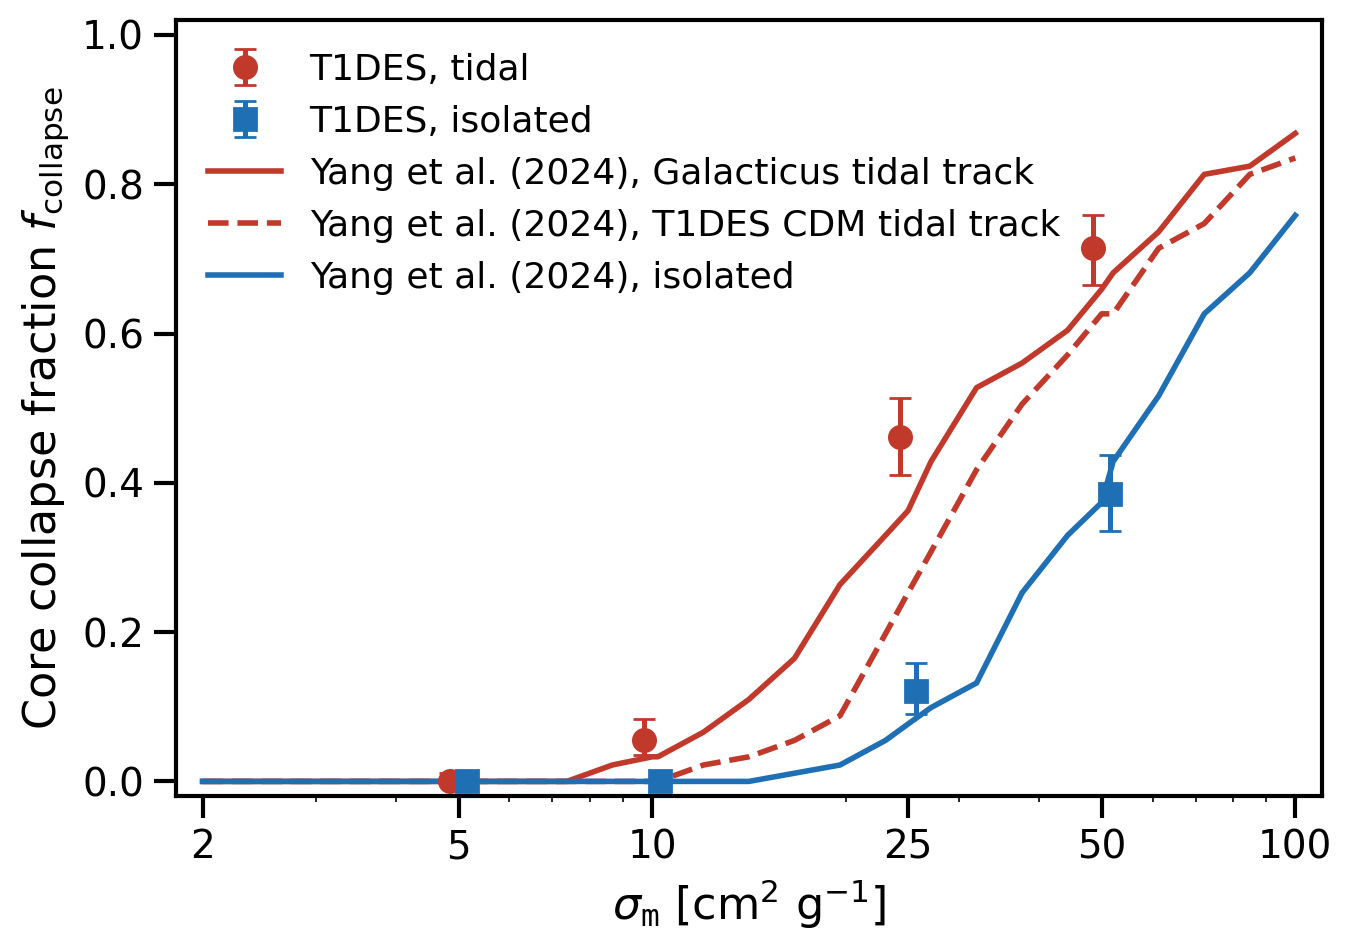
\includegraphics[width=0.5\linewidth]{figures/collapse_fraction_vs_sigma_paper_scratch.png}
    \caption{
             The cross section per unit mass vs the core collapse fraction for our \tides simulations compared to as well as predictions from \cite{yang2024parametric}. In red: results from our t1des subhalo simulations (red dot with error bars), and the Yang models integrated over the the tidal tracks from \gal (red solid) and from the \tides CDM (red dotted) in blue. We find our \tides model is fairly consistent with the predictions from the \cite{yang2024parametric} model, though our \tides model may predict slightly higher fractions of core collapsed halos. In blue is the results for the isolated case, if the subhalos remained isolated, what fraction would collapse? Our \tides model is consistent with the predictions of the Yang model here and predicts strictly lower collapse fractions for isolated halos. No halos collapse in the field that also do not collapse as a subhalo.              
    }
    \label{fig-collapse}
\end{figure*}

\section{Conclusion and Summary}\label{sec-conclusion}

In this work, we have presented \tides, a novel method of simulating SIDM subhalos using a modified version of the \nsphere 1D N-body code.
Here we provide a summary of this work. 
In \refsec{sec-methods} we discuss the methods used in this paper in three subsections. 
First, in \refsec{sec-realizations} we discuss the \gal model used to obtain the mass histories used by \tides and the initial conditions used in our \tides simulations. 
Then in \refsec{sec-dynamics} we discuss the dynamics implemented in our fork of \nsphere; in particular we focus on the tidal physics implemented in our simulations: a linear effective tidal field, calculated in a CDM first pass to match the mass history of a target subhalo.
Thirdly, in \refsec{sec-sidm} we give an overview of the SIDM physics implemented in NSphere and discuss our core collapse conditions for subhalos. a
In the main section,  \refsec{sec-results} we discuss the main results from this work: with no evaporation, find that a tidal field strictly accelerates accelerates core collapse; and that this acceleration is cross section dependent and significant: up to a factor of nearly $4$ time the number of subhalos collapse when compared to their isolated counterparts. 
Finally, here we discuss future work, discuss some potential caveats and provide concluding statements. 

To correctly infer constraints on SIDM models through lensing studies, it will be important to thoroughly understand predicted core collapse rates.
Our model gives a distinct advantage here: because it is much more computationally efficient than previous SIDM simulations, by making modifications to our pipeline it may now be practical to test a wider range of parameter and model space within SIDM. 
In addition to more thoroughly exploring the parameter space of specific SIDM due to the reduction of computational cost in our simulations 
By making some modifications to our code it is possible to explore a wide range of velocity and angle dependent cross sections.
By adding in stochastic scattering chance of a particle interaction with the host simulating evaporation is possible within our model; we leave exploration of this to future work. 
Additionally, \nsphere is not limited to dark matter only physics; it may be interesting to explore the effect of a central galaxy on core collapse times. 

Our \tides model is in reasonable agreement with \gal the tidal tracks of \gal halos, however some outlier halos disagree on order $50 \%$ of $V_{\tt max}$; this disagreement is particularly pronounced for subhalos that are early in their evolution. 
This may be due to the initial conditions used by N-Sphere and the non physical stair stepping mass histories predicted by \gal.
It may be worth further exploring seeding the \tides pipeline with N-body mass histories rather than \gal mass histories. 
We o not include any pre-infall SIDM evolution in our models; depending on the cross section, pre-infall SIDM evolution may be significant enough to form a core that effects the tidal physics of the subhalo.
We leave investigating this regime to future work. 

In conclusion, by simulating SIDM subhalo evolution in 1D, we are able to be much more computationally efficient in simulating SIDM subhalos when compared to traditional 3D N-body simulations by over an order of magnitude; our simulations are able to be simulated on a laptop and  ran in the span of hours (this is greatly particle count and thus mass loss dependent).
We shared 
Previous 1D SIDM subhalo simulations relied on coarse approximations of tidal stripping, such as approximating the tidal stripping as per orbit truncations to the mass profile; we include a much more realistic mass profile that reasonably approximates the mass history over time as well as the internal $R_{\tt max}$ and $V_{\tt max}$ properties of the subhalo. 
We find that under our assumption of no evaporation, subhalo core collapse is strictly accelerated when compared to isolated field halos. 
Additionally, we find that our simulations are in broad agreement with the \citet{yang2024parametric} parametric model. 

\begin{acknowledgments}
We wish to acknowledge the support of the author community in using
REV\TeX{}, offering suggestions and encouragement, testing new versions,
\dots.

Generative AI Discolusure --- Generative AI (LLMs) were used in some portions of the research process for this work.
Several Claude models were used as a part of this project: Claude Haiku, Sonnet, Opus and Fable\footnote{Many versions of Claude models were used throughout the project, starting at version 4.5 for haiku,sonnet and opus through to version 5.1 of fable} were used for coding assistance (including the generation of plots), summarization of background literature, as a general learning tool, transcriptions (taking an image of a diagram drawn by pencil and converting it to latex) and for several discussions about the project.
We disclose that coding agents were used for several portions of this project such as writing portions of the tidal physics model, packaging \tides into an ergonomic command line utility, implement various features into tides such as the "smoothed" and "isolated" modes, various assistance with analysis such as the generation of the figures in this work. 
Generative AI was also used for summarization of literature and as a general learning tool "E.X What are the ways core collapse in previous SIDM works?".
Generative AI was not used in the writing of this manuscript. 
For some early exploratory work, discussions and brainstorming with AI was tested "E.x What are some ideas for figures?". 
However, this usage was found to be infective and for this manuscript nearly all useful AI assistance was directed coding tasks, literature summarization, transcription and as and as a learning tool.
We verify the output from AI coding agents in several ways: code generated by agents was reviewed, tests suggested by both agents and humans were set up and manually reviewed by the authors and finally, for a variety of tasks was duplicated and key results were checked by human made programs. 


\end{acknowledgments}

\appendix

%\section{CDM Tidal Physics}\label{apdx-tidal}
%Here, we discuss the results of our CDM simulations. 
%We show mass histories and tidal tracks for a sample of NSphere subhalos (for both the tidal field calculation runs and using a smoothed tidal field) and their \gal halo counterparts. 
%
%Mass history --- We note that mass vs time plots have excellent agreement with \gal; this is not surprising as we calculate a tidal field to match the galacticus mass history. There are some exceptions -- our tidal stripping model "over strips" in some cases and fails to catch back up to \gal. This is particularly visible for subhalos with sections of very steep mass loss. 
%
%Smoothed vs unsmoothed tidal field --- We note that the tidal field smoothed with a gaussian filter of width $0.1 T_{\tt dyn}$ is visually smooth for all halos the sharp spikes seen in the unsmoothed tidal field are completely gone. The evolutionary histories of the smoothed and unsmoothed tidal fields are almost identical for a smoothed tidal field.. 
%
%TSMOOTHEDidal Tracks --- Nsphere and \gal agree well on the tidal tracks of the subhalo; while our model calculates a tidal field that aproximates the mass history of the galacticus subhalo, the tidal tracks are not taken into account in this process -- even so we are able to reproduce (to good aproximation) the galactus tidal tracks. 


%\section{Convergence testing}
%BLAH BLAH BLAH

% The \nocite command causes all entries in a bibliography to be printed out
% whether or not they are actually referenced in the text. This is appropriate
% for the sample file to show the different styles of references, but authors
% most likely will not want to use it.
\nocite{*}

\bibliography{t1des}% Produces the bibliography via BibTeX.

\end{document}
%
% ****** End of file apssamp.tex ******
